% \chapter{Visual-linguistic Semantic Correspondence from Weak Supervisions}
\chapter{VL SEMANTIC CORRESPONDENCE FROM WEAK SUPERVISIONS}


Visual recognition understands the content of image by categorizing the target object from pre-defined classes. Treating such problem as a classification task narrows the scope of what machines can recognize due to the limited data and computing power.
Language, however, contains large-scale and plentiful textual descriptions about the attributes, states, or even underlying aspects about the target object or scenes. For example, the textual phrase ``\textit{a boy in blue shirt}'' does not only implies of the existence of person, while also indicating the gender, age and the color of the dress on the target object. The utilization of open-form sentences enables the grounding system to localize object in a greater scope and flexibility. 
Though textual description does not always precisely and comprehensively covers the content of the image, such data always couples with ``large-scale'' and ``weak'' labels. This chapter studies how to better leverage and exploit textual data as weak supervision and find the image region (or video moment) that best matches the textual descriptions when no bounding box (or temporal boundary) annotations.
This chapter contains several works for the textual grounding on image, video moment/activity localization by language tasks all in a weakly-supervised learning fashion for semantic correspondence capturing.

\section{Associating V to L without Explicit Supervisions}
Multi-modal tasks, \eg. assistive visual search~\citep{cai2004hierarchical, la1998combining}  and image captioning~\citep{you2016image, vinyals2017show}, has been studied for decades in the community. While those tasks are classical topics in computer vision and natural language processing,
current advancement has further energized it by interplaying
vision (images) and language (high-level guide) for practical applications. Specific examples include referring expressing understanding~\citep{nagaraja2016modeling,hu2017modeling} and reasoning-aware visual-question-answering~\citep{hu2017learning}.

State-of-the-art textual grounding methods \citep{yu2018mattnet, hu2016natural, rohrbach2016grounding, plummer2015flickr30k, yeh2017interpretable, luo2017comprehension, fang2018weakly} are based on deep neural networks and relying on
large-scale training data with manual annotations for the object bounding box and relationship between
phrases and figures/objects.
This setup largely limits their broad applications as such strong supervision is expensive to obtain,
and they also lack interpretability and resilience to counterfactual cases which do not appear in training.




\section{Weakly-Supervised Textual Grounding on Images}

\begin{figure*}[h]
  \begin{center}
    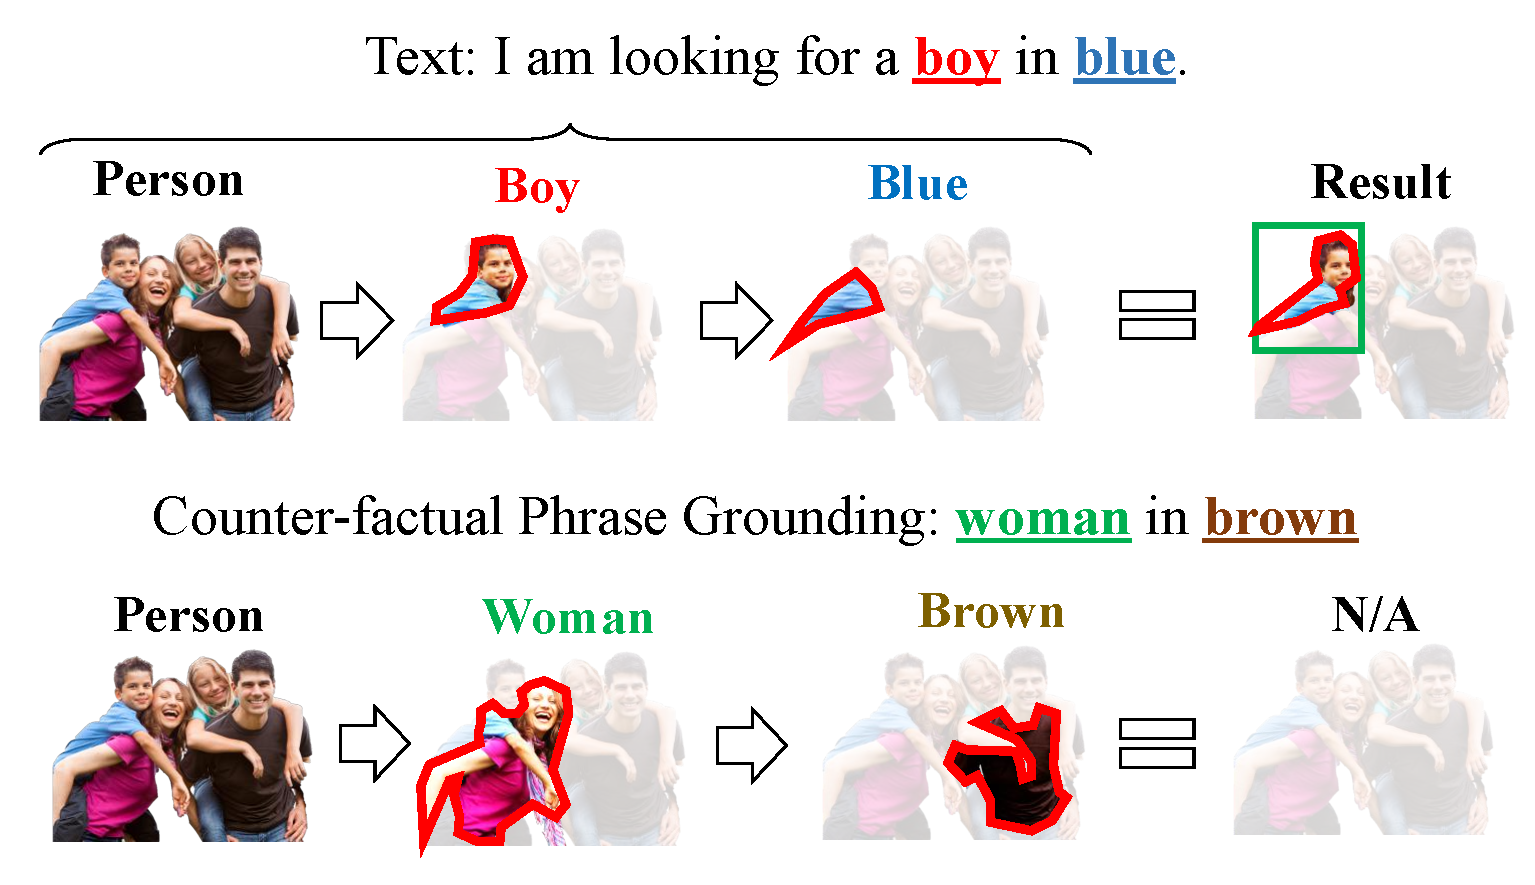
\includegraphics[width=1.0\textwidth]{images/mtg_abstract.pdf}
  \end{center}
  \caption{A example of textual grounding system, where the visual concepts are localized by open-form textual description, thus enabling the system to interact with users with high flexibility.}
  \label{fig:grounding}
 \end{figure*}

Computer Vision applications often require a textual grounding module with precision, interpretability, and resilience to counterfactual inputs/queries. To achieve high grounding precision, current textual grounding methods heavily rely on large-scale training data with manual annotations at the pixel level. Such annotations are expensive to obtain and thus severely narrow the model's scope of real-world applications. Moreover, most of these methods sacrifice interpretability, generalizability, and they neglect the importance of being resilient to counterfactual inputs. To address these issues, we propose a visual grounding system which is 1) end-to-end trainable in a weakly supervised fashion with only image-level annotations, and 2) counterfactually resilient owing to the modular design. Specifically, we decompose textual descriptions into three levels: entity, semantic attribute,  color information, and perform compositional grounding progressively. We validate our model through a series of experiments and demonstrate its improvement over the state-of-the-art methods. In particular, our model's performance not only surpasses other weakly/un-supervised methods and even approaches the strongly supervised ones, but also is interpretable for decision making and performs much better in face of counterfactual classes than all the others.


\begin{figure*}[t]
\begin{center}
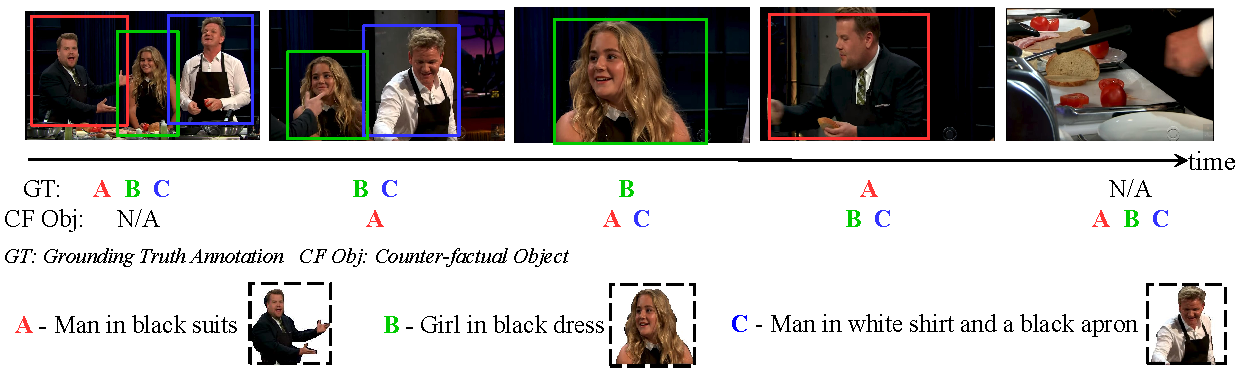
\includegraphics[width=1.0\linewidth]{images/ca_demo.pdf}
\end{center}
\caption{Example of the counter-factual object grounding.}
\label{fig:ca_demo}
\end{figure*}


\subsection{Modularized Textual Grounding Model with Weakly-supervised Training}
To obtain better interpretability and counterfactual resilience,
we propose to modularize the our whole textual grounding system
by decomposing the textual descriptions into multiple levels,
each of which is passed to a specific module to process.
We generate the final grounding result by progressively merging intermediate
results from these modules.

Without losing generalization,
in this work,
we decompose the textual descriptions into three levels,
and progressively process them with three different modules, respectively:
entity grounding module $M_e$,
semantic attribute grounding module $M_a$, and color grounding module $M_c$.
We extracted phrases and words that belong to such three levels from text, and feed them into their corresponding sub-modules.
We note that such a modular design allows for training different modules using different specialized protocols,
e.g., fully supervised learning or weakly supervised learning,
while also enables end-to-end training.
For the final grounding heat map $G$,
we merge progressively the intermediate results from these modules as below (see Figure \ref{fig:pipeline}):
\begin{equation}
\begin{split}
G & = M_e \cdot (M_a + M_c).
\label{eq:att}
\end{split}
\end{equation}

In practice, we observe that such a merging approach achieves the best
performance, better than the straightforward multiplicative or additive fusion.
This is because that the entity grounding sets the object constraints, and the summation
over the attribute and color modules interpretably delivers how the final results are generated,
though they may partially cover some regions belonging to the object of interest.
In the remaining of this section,
we elaborate each of the three modules and the adopted training protocols.



\subsubsection{Entity Grounding Module (M$_{e}$)}


\begin{figure*}[t]
\begin{center}
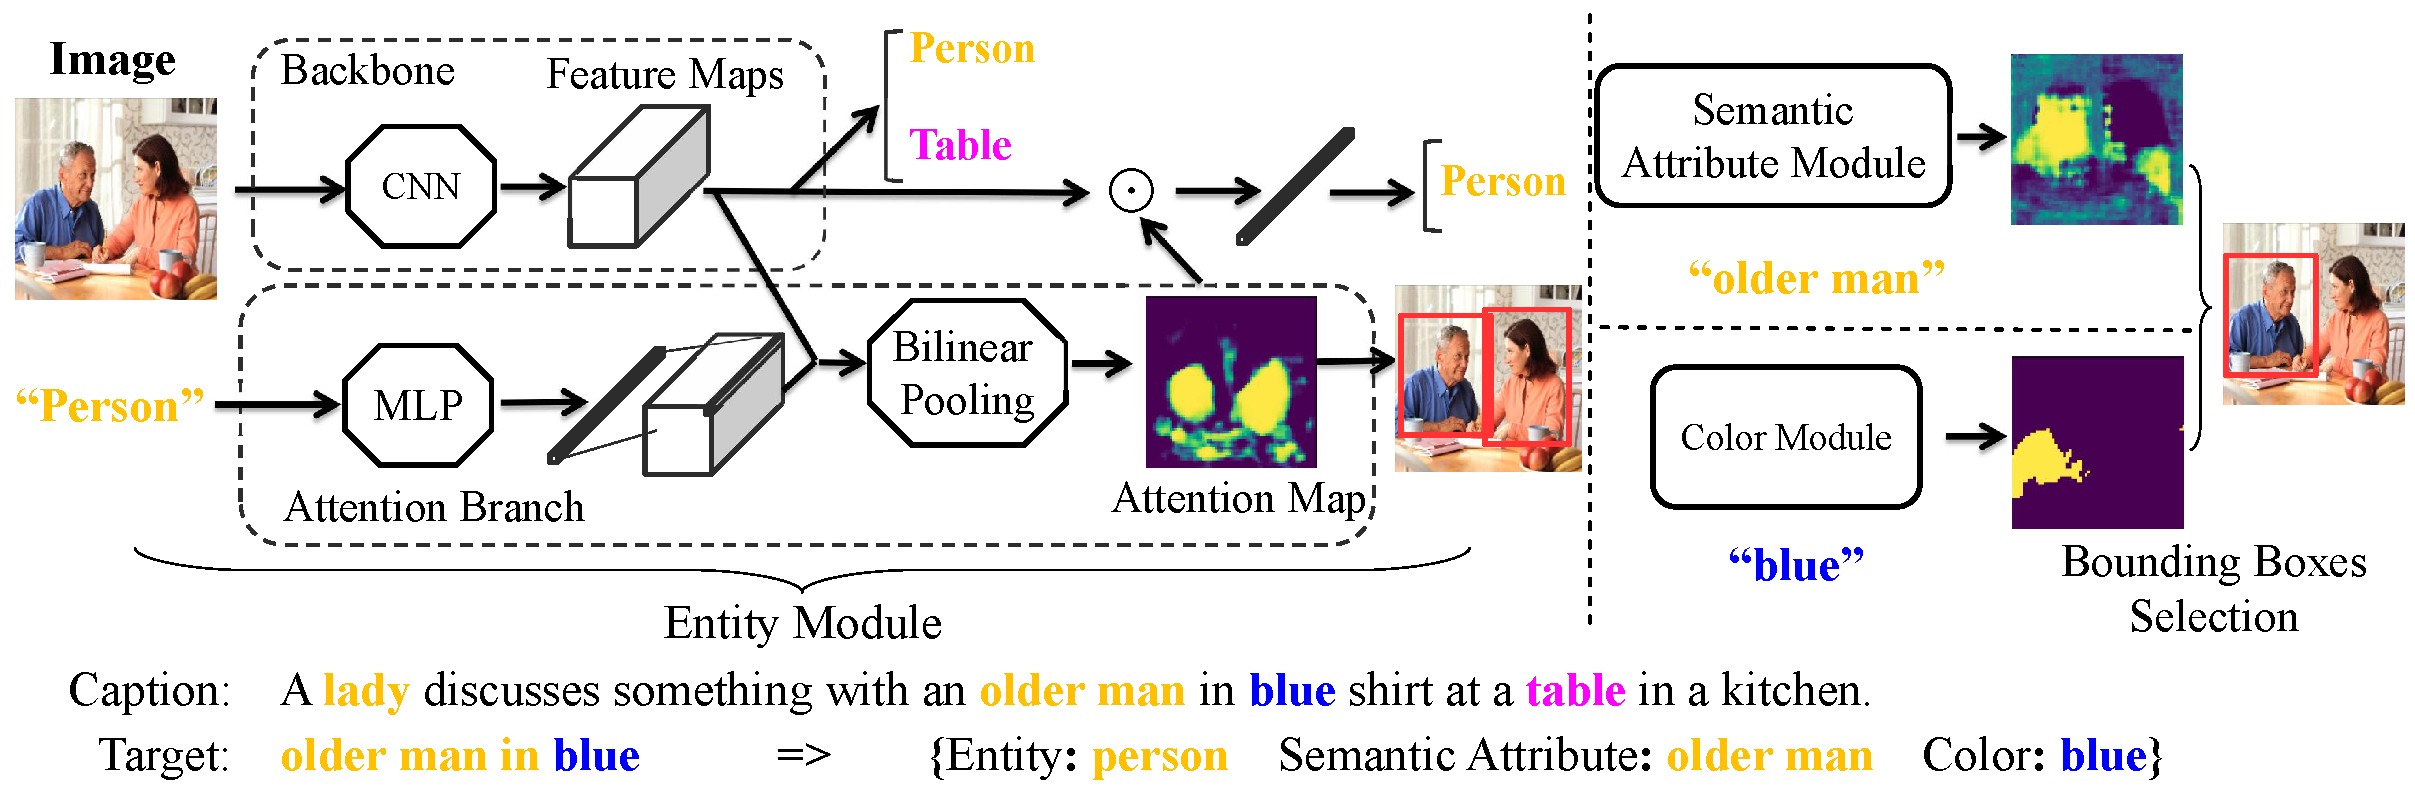
\includegraphics[width=1.0\linewidth]{images/pipeline.pdf}
\end{center}
\caption[Illustrative diagram for our entity grounding module (left) and the whole
textual grounding system(right).]{Illustrative diagram for our entity grounding module (left) and the whole
textual grounding system (right). The textual phrase is first decomposed into sub-elements, e.g., ``older man in blue" can be parsed to ``person'' category with ``older man'' and ``blue'' to be it's attributes, and later fed into corresponding sub-module. The bounding boxes are generated and selected based upon the merged attention maps. We train the entity/semantic attribute grounding module in a weakly supervised fashion with a attention mechanism. The semantic attribute module also adopt similar architecture of entity module, however with a dictionary learning loss. (best viewed in color)}
\label{fig:pipeline}
\end{figure*}


To overcome the limitation of current methods that require expensive manual annotations at fine-grained level,
we propose to train the entity grounding module in a weakly supervised learning manner.
This can help our system achieve better generalizability to other novel data domains which may just require fine-tuning over dataset annotated coarsely at image level.
This weakly supervised learning can be expressed as selecting the best region $r$ in an image $I$ given an object of interest represented by a textual feature $t$, e.g., a word2vec feature.
With well pre-trained feature extractor, we first extract visual feature maps $v$ over the image, 
based on which we train an attention branch $F$ that outputs
a heatmap expected to highlight a matched region in the image. 

Mathematically, we are interested in obtaining the region $R = F(t, v)$ in the format of heatmap and making sense of it. In practice, we find training a classification model at image level with the attention mechanism works well for entity grounding, which is the output through the attention maps, as illustrated by Figure~\ref{fig:pipeline} left. Moreover, rather than using a multiplicative gating layer to make use of the attention map, we find that it works better by using a bilinear pooling layer \citep{lin2015bilinear,gao2016compact,kong2017low}.

For bilinear pooling, we adopt the Multimodal Compact Bilinear (MCB) pooling introduced in~\citep{fukui2016multimodal} that effectively pools over visual and textual features. In MCB, the Count Sketch projection function \citep{charikar2002finding} $\Psi$ is applied on the outer product of the visual feature $v$ and an array repeating the word feature $t$ for dimensionality reduction: $\Psi (t)\ast \Psi(v)$. If converted to frequency domain, the concatenated outer product can be written as: $\Phi= {FFT}^{-1}(FFT(\Psi (t))\odot FFT(\Psi(v)))$. Based on $\Phi$, the final 2D attentive map $R$ is computed through several nonlinear 1$\times$1 convolutional layers : $R$ = $conv(\Psi)$, with the final one as sigmoid function to shrink all values into $[0,1]$. Later we retrieve the regional representation $f$ by a global pooling over the element wise product between entity attentive map and original visual feature maps: $f = pool(R\odot v)$, on which the weakly supervised classification loss is applied.
Overall, to train the entity grounding module with the attention mechanism in a weakly supervised learning fashion,
we train for image-level $K$-way classification using a cross-entropy loss.



\subsubsection{Semantic Attribute Grounding Module (M$_{a}$)}
The semantic attribute grounding module improves interpretability of the whole textual
grounding system by explaining that it explains how the final decision is being made. For example, a model finding the ``man in black suits'' as shown in Figure~\ref{fig:ca_demo} should not only output the final grounding mask, but also explain how the final result is being achieved by showing where ``man'' and ``black suits'' are localized in the image.

We also train this module with a weakly supervised learning protocol with similar architecture in the entity module.
But instead of training with $K$-way classification over $K$ predefined attributes as in training entity grounding module, we model this as a multi-label problem, since an image may deliver multiple attributes which are not exclusive to each other. Moreover, rather than classifying them, we propose to use regression for training, since attributes can become large in number while the features representing attribute names can lie in a manifold in the semantic space. This makes our module extensible to more novel attributes even trained with some pre-defined ones.

Note that we represent each attribute with the word2vec feature \citep{mikolov2013distributed}.
Although the word2vec model demonstrates very semantic grouping on words,
we find that these features representing attributes do not deliver reasonable discriminativeness. For example, in word2vec features,
``man'' is more similar to ``woman'' than ``boy'' but we care more about the gender meaning in practice.
Though retraining such a word2vec model solves the problem,
we adopt an alternative method in this paper by proposing a dictionary based scoring function
over the original word2vec features.
We note that this method not only offers more discriminative scoring power,
but also inherits the semantic manifolds in word2vec features,
extensible to novel attributes without re-training whole model as done in $K$-way classification.

To introduce our dictionary based scoring function,
we revisit the classic logistic normalization widely used in binary classification as below:

\begin{equation}
	y_i = \frac{1}{1+\exp(-\w_i^T\x)}
\end{equation}

where ${\bf w}_i$ here represents the learning parameters, 
and ${\bf x}, y_i$ are the input vectors and predicted probability with respect to class $i$.
Note again that, although the logistic loss works well for binary classification
or multi-label classification,
it is not extensible to novel classes unless retraining the whole model.
Our solution to this is based on the proposed dictionary based scoring function.
Suppose there are $C$ attributes, represented by word2vec and stacked as a dictionary
${\bf D}=[{\bf d}_1, \dots, {\bf d}_C]$.
We can measure the (inverse) Euclidean distance between $\x$ and each dictionary atom
for the similarity about which attribute $\x$ is predicted.

So the dictionary acts as the parameter bank
which can be fixed if we want to preserve the
semantic manifold in the word2vec feature space,
and we have the following modified sigmoid transformation:
\begin{equation}
	y_i = \frac{2}{1+\exp(\Vert{\bf d}_i-\x\Vert_2^2)}	
\end{equation}
However, as this may also be less discriminative,
we opt to learn a new latent space.
Concretely, we build new layers before the sigmoid transformation,
and these layers form new function $\phi$ and $\psi$
to transform the feature $\x$ and dictionary atoms, respectively.
Then we have the following dictionary based scoring function for the $i^{th}$ attribute:
\begin{equation}
	y_i = \frac{2}{1+\exp(\Vert \psi({\bf D})_i - \phi(\x)\Vert_2^2)}	
\end{equation}


Furthermore,
despite using the dictionary based scoring function as a modified sigmoid for logistic loss over
the holistic feature globally pooled over the image,
we also perform it at pixel levels.     % as in~\citep{kong2018recurrent}.
Concretely,
during each iteration on each training image,
we choose the $T$ pixels with the top scores to feed into the logistic loss.
This practice is essentially a multi-instance learning at pixel level ~\citep{paul2018w}.
We find in our experiment that jointly using the two losses helps generate
better attention maps.



\subsubsection{Color Grounding Module (M$_{c}$)}
When querying in natural languages,
human beings typically rely on textual descriptions for low-level vision characteristics,
e.g., color, texture, shape and locations.
Recent work also demonstrates the feasibility of grounding low-level features in unsupervised learning~\citep{vondrick2018tracking}.
In our work for the datasets we studied in our work,
we notice that color is the most used one.
In the Flickr30k Entities dataset~\citep{plummer2015flickr30k} as studied in this paper, 
70\% attributes words are colors describing persons. 
Therefore, 
without loss of generalization, 
we propose to build a separate color grounding module to
improve the interpretability of the whole textual grounding system.


Different from entity grounding and semantic attribute grounding modules,
we train this color grounding module in a fully supervised way over a small-scale dataset, called Color Name Dataset~\citep{van2007learning},
which contains 400 images with color name annotations at pixel level.
We essentially perform pixel-level color segmentation over the input image
to ground color reference. Moreover, we build this color grounding module over a ResNet50 model~\citep{he2016deep} pretrained on ImageNet dataset~\citep{deng2009imagenet}, and concatenate intermediate features at lower levels for pixel-level color segmentation. We find this works better than combining high-level features. We conjecture the reason is due to that color is a very low-level cue that does not require deep architectures and high-level feature abstraction. This is consistent with what reported in \citep{larsson2016learning}.





\begin{figure*}[t]
\begin{center}
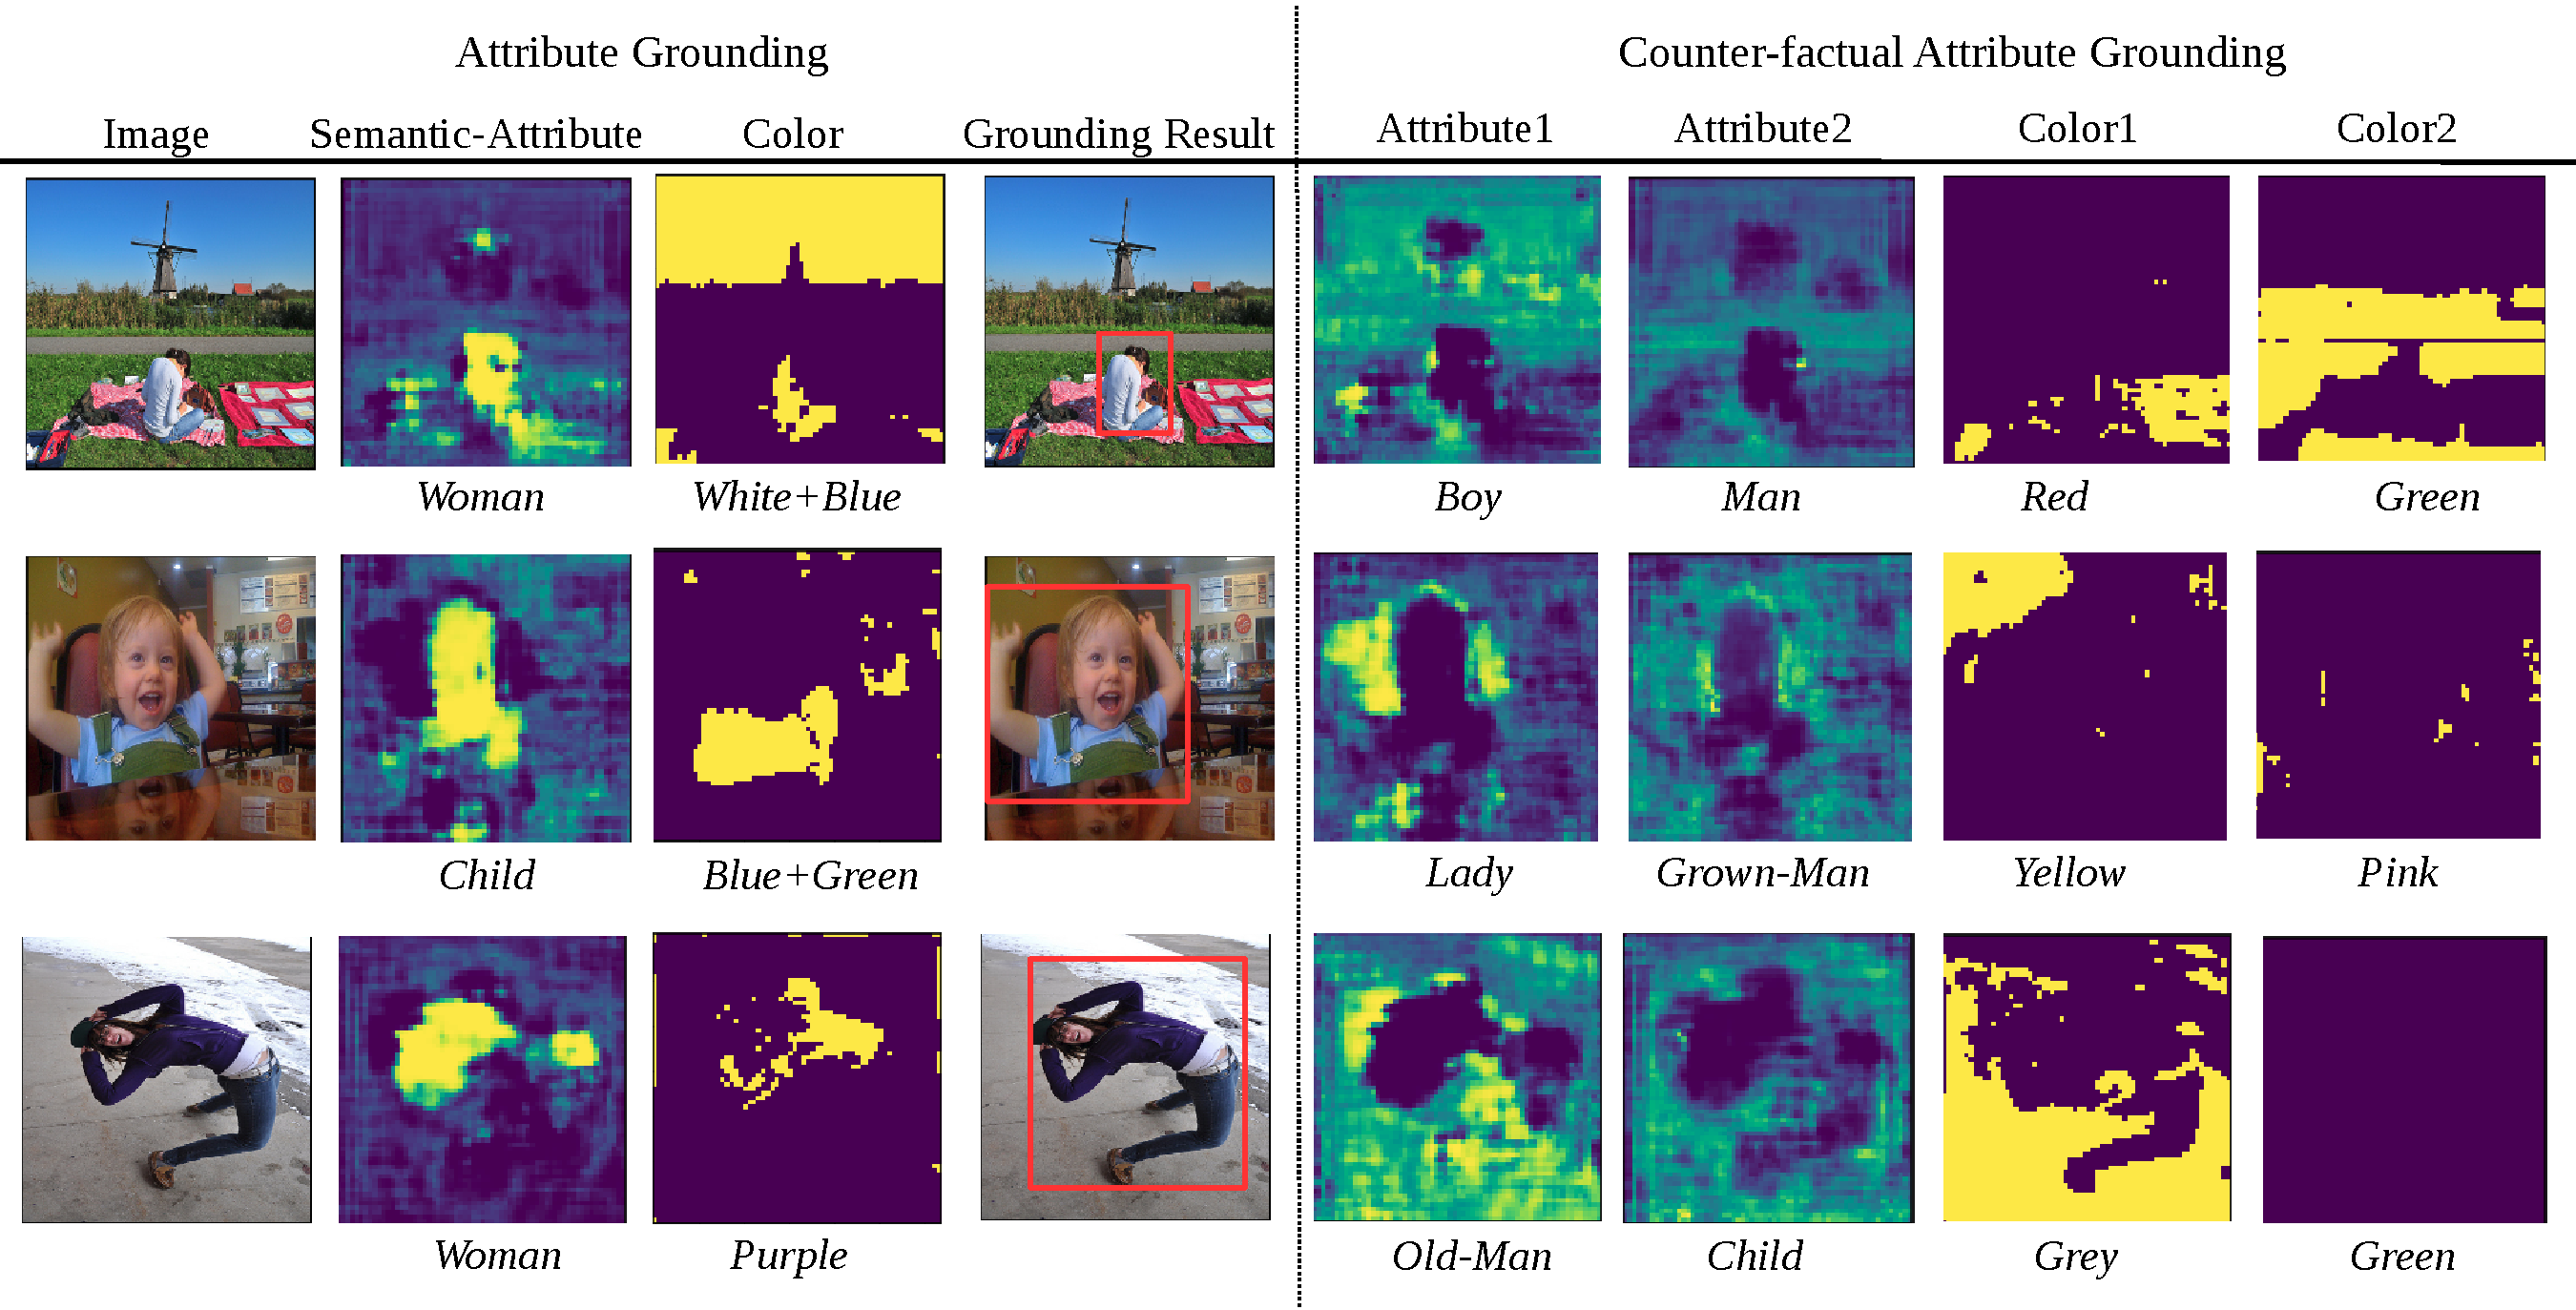
\includegraphics[width=1.0\linewidth]{images/qualitative.pdf}
\end{center}
\caption{Examples of attribute grounding predictions (left) and counterfactual attribute grounding results (right). (best viewed in color) }
\label{fig:demo}
\end{figure*}



\subsubsection{Architecture and Training}
Our three modules are based on the ResNet architecture~\citep{he2016deep}.
Similar to~\citep{chen2018deeplab,kong2017recurrent}, we increase the output resolution of ResNet
by removing the top global $7\times 7$ pooling layer and the last two $2\times2$
pooling layers, replacing them with atrous convolution with dilation rate 2 and
4, respectively to maintain a spatial sampling rate.
Our model thus outputs
predictions at $1/8$ the input resolution which are upsampled for benchmarking.
For (multi-label or $K$-way) classification,
we use a global pooling layer that produces a holistic image feature for classification.
In addition, we also insert an $L_{2}$ regularization over the attention maps,
and we observe that such a regularization term helps reduce noises effectively.

We use the standard stochastic gradient decent (SGD) for training in a stagewise fashion.
Specifically,
we first train a plain classification model for entity and semantic attribute grounding modules,
then we build the attention branch for attentional learning.


Though our textual grounding system is end-to-end trainable,
we train each module separately.
And though joint training is straightforward to implement,
we do not do this for practical reasons:
1) we can easily plug in a better trained module without retraining the whole system
for better comparison; 2) we focus on the modular design,
isolating the influence of the settings and parameters of each module.


\begin{figure}[h]
\begin{center}
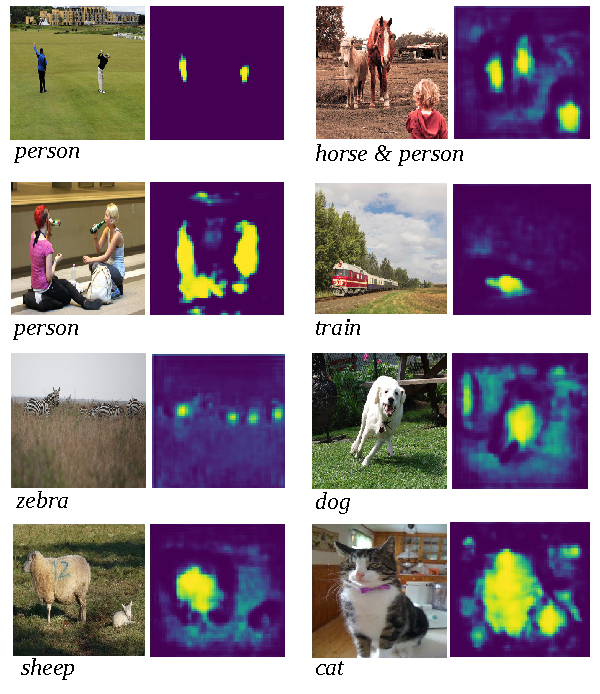
\includegraphics[width=.95\linewidth]{images/entity_demo.pdf}
\end{center}
\vspace{-7mm}
\caption{Qualitative examples of attention maps from the entity module.  }
\vspace{-5mm}
\label{fig:entity_demo}
\end{figure}


\subsection{Experiment}
We now experimentally validate our system and compare it with the state-of-the-art methods.
To highlight the generalizability of our system,
we train it on COCO2017 dataset~\citep{lin2014microsoft}
while test it on another Flickr30K Entities dataset~\citep{plummer2015flickr30k}.
We first introduce the two datasets briefly before conducting thorough comparisons,
then we carry out another experiment to show our (weakly supervised) model performs remarkably better than other (fully supervised) methods on a collected dataset consisting of counterfactual testing cases.


\subsubsection{Datasets and Preprocessing}
The two datasets we used in our experiments are:
COCO2017~\citep{lin2014microsoft} for training our system
and Flickr30k Entities Dataset \citep{plummer2015flickr30k} for testing it.

COCO2017 dataset contains 110k training images with 80 object categories at image level.
These 80 object categories are used for training our entity grounding module as they can be
seen exclusive to each other.
The captioning task and the annotations provided in COCO2017 enables us to train
our semantic attribute grounding module. Using \citep{bird2009natural,miller1998wordnet}, we tokenize and mine out words related to semantic attributes
(e.g., man, woman, boy, old and young) to form our corpus.
To train the semantic attribute grounding module,
we retrieve images from COCO2017 whose captions contain the attributes existing in our corpus.
Eventually,
10,000 images and 34 attributes are collected from COCO2017 for weakly supervised training our modules.
To alleviate imbalanced distribution of these attributes,
we adopt inverse frequency reweighting during training.

The Flickr30k Entities dataset contains over 31k images with 275k bounding boxes with natural languages descriptions,
and we only use this dataset for testing our system with the bounding boxes.

To carry out counterfactual testing experiment,
we collect a new testing set with images from Flickr30k and RefCOCO+ \citep{kazemzadeh2014referitgame}.
The images only contain persons and relevant attributes (e.g., gender, age, etc),
so we call this dataset Person Attribute Counterfactual Grounding dataset (PACG).
By developing an easy-to-use interface,
we are able to generate counterfactual captions for a given image with the good captions provided by the original dataset. Similar to work in \citep{hendricks2018generating}, we generate counterfactual attributes by mining the negation of existing attributes. The overall PACG dataset consists 2,000 images,
a half of which are with counterfactual attributes not existing in the image
and the other half with ``correct'' attributes.


\noindent{\bf Language Processing:}
To deal with free-form textual queries,
we use a language parser ~\citep{bird2009natural} to select the keywords according to the functionalities of the three modules.
We first extract the entity words and pick the most similar object classes by word similarities.
We then extract the semantic attribute words in the same way.
Finally, we extract the the color keywords simply for the color grounding.
%Furthermore, according to the word frequence statistics on Flickr 30k \citep{plummer2015flickr30k}, 70\% of the remaining semantic attribute words are related to person and colors. Thus we restricted our semantic dictionary to only human-related visual properties together with color informations. We pick  25 human-related attributes words that mainly cover the gender and age attributes.
To represent the textual attributes and color names,
we adopt the word vectors from GloVe \citep{pennington2014glove}.
This enables meaningful similarity between the defined attributes/colors and
novel ones when encountered at testing stage.
%\TODO{When constructing semantic attribute dictionary, we refer to the WordNet~\citep{miller1998wordnet} and compute word to attribute similarities among each word-attribute pairs.}%




\newcommand\Tstrut{\rule{0pt}{2.2ex}}        
\newcommand\Bstrut{\rule[1.6ex]{0pt}{0pt}} 

\begin{table}[htbp]
\begin{center}
\caption{Phrase localization performance on Flickr 30k Entities (accuracy
in \%). }
\begin{tabular}{c c c}
\toprule
Aprroach & Image Features & mAP (\%)\\
\hline
\textbf{Supervised} \Tstrut\\
SCRC \citep{hu2016natural} & VGG-cls & 27.80\\
GroundeR$_{s}$ \citep{rohrbach2016grounding} & VGG-cls & 47.81\\
CCA \citep{plummer2015flickr30k} &  VGG-det & 50.89\\
IGOP \citep{yeh2017interpretable} &  YOLO+DeepLab & \textbf{53.97}\\
\hline
\textbf{Unsupervised} \Tstrut\\
Largest proposal & n/a &  24.34\\
GroundeR$_{u}$ \citep{rohrbach2016grounding} & VGG-det & 28.94\\
Mutual Info. \citep{zitnick2013learning} & VGG-det & 31.19\\
UTG \citep{yeh2018unsupervised} & VGG-det & 35.90\\
UTG \citep{yeh2018unsupervised} & YOLO-det & 36.93\\
\hline
\textbf{Weakly-Supervised}\Tstrut\\
Ours$^{1}$  & Res101&  29.01\Tstrut\\
Ours(Attr)   & Res101& 32.04\\
Ours(Attr+Col)  & Res101& 33.43\\
Faster-RCNN~\citep{ren2015faster} & Res101-det& 35.35\\
Ours+Attr   & Res101-det& 47.46\\
Ours+Attr+Col  & Res101-det& \textbf{48.66}\\
\bottomrule
\end{tabular}
\end{center}
\label{table:flickr}
\end{table}



\subsection{Result}
We compare our modular textual grounding system with
other supervised/unsupervised methods on the Flickr30k Entities dataset.
We use the mean average precision (mAP) metric to measure the quantitative performance.
The detailed comparison is listed in Table~\ref{table:flickr}.

As the first baseline method similar to~\citep{yeh2018unsupervised},
we select the largest proposal as the final result.
This method achieves 24.34\% mAP.
Then, we build another baseline model that
we train the entity grounding module only through weakly supervised learning over a ResNet101 backbone, which is pretrained over ImageNet dataset. Then, over the entity grounding heatmaps,
we generate bounding boxes candidates by sub-window search \citep{lampert2009efficient} together with contour detection results, followed by a Non-Maximum Suppression to further refine the proposal boxes. We select the box that encompasses largest ratio of object according to equation \ref{eq:att}. We note that this simple baseline module (29.01\% mAP) outperforms GroundR$_{u}$~\citep{rohrbach2016grounding} (28.94\% mAP) that learns grounding in an attentive way over large-scale training data.
If we include our semantic attribute module,
we improve the performance further (32.04\% mPA),
outperforming Mutual Info.~\citep{zitnick2013learning}. If we further insert the color grounding module,
we achieve comparable performance (33.43\%) to UTG (36.93\% mAP),
which adopts an unsupervised method to link image concepts to query words~\citep{yeh2018unsupervised}.
We note that our models are trained on COCO dataset only,
unlike all these methods which are trained on the same dataset (Flickr30k dataset).
The effectiveness of our model is demonstrated by its good transferability, as it is trained and tested
on different data domains.


\begin{figure}[t]
\begin{center}
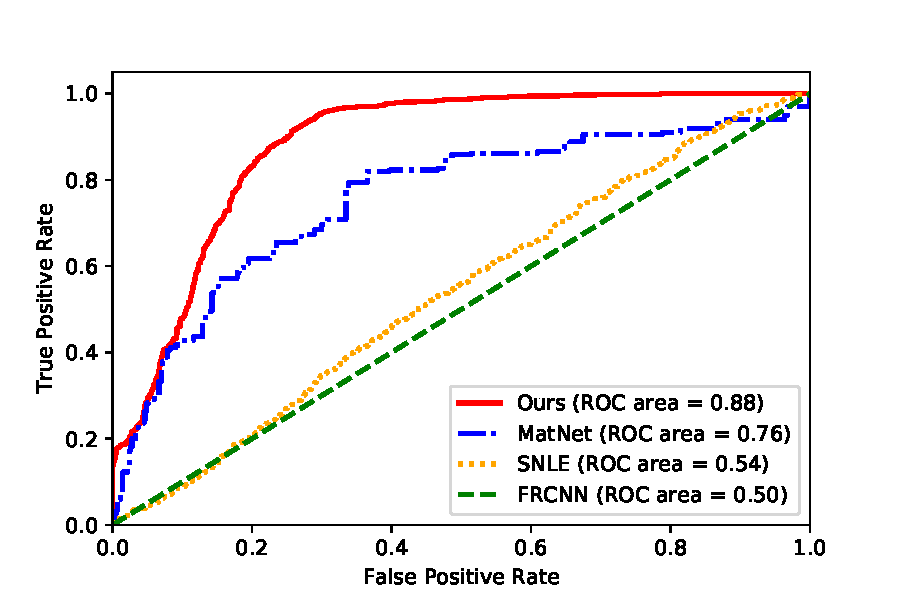
\includegraphics[width=1.1\linewidth]{images/roc}
\end{center}
\caption{ROC of our modular network demonstrates high resolving ability on PACG dataset with an AUC of 0.88, comparing to other state of the art baseline models (best viewed in color).  }
\label{fig:roc}
\end{figure}

It is also worth noting that, all the compared unsupervised methods unanimously adopt a well-trained object detector, even though they claim to be unsupervised learning.
To gain an idea how the detector improves the performance,
we fine-tune the faster-RCNN detector~\citep{girshick2015fast} on COCO
and train our modules with weak supervision again.
We report our results as the bottom two rows in Table \ref{table:flickr}.
Now we can see our models perform significantly better, and even surpasses some fully supervised methods (SCRC~\citep{hu2016natural}
and GroundeR~\citep{rohrbach2016grounding}).
Although it seems unfair that our system adopts ResNet101 architecture
while most compared methods uses shallower VGG networks,
we note that IGOP which adopts both VGG and ResNet101 (denoted by DeepLab) 
achieves the best performance with fully supervised training.
Even though our best model does not outperform IGOP,
we believe the performance gap is small and reasonable as our training is carried out
on a different dataset (COCO) rather than Flickr30k, and it does not
rely on any strong supervision signals. We show output examples of entity grounding module in Figure \ref{fig:entity_demo} with various object categories as input, and attribute grounding outputs in Figure \ref{fig:demo}, with both existing attributes and counterfactual attributes as queries. These visualizations demonstrates how our system rejects  in an explainable way the counterfactual queries through the modular output.

\subsubsection{Counterfactual Grounding Evaluation}
We now carry out in-depth study on how our system performs when facing of counterfactual textual queries over our collected
PACG dataset, and compare with three baseline or state-of-the-art methods, Faster-RCNN~\citep{ren2015faster}, MattNet \citep{yu2018mattnet}, SNLE \citep{hu2016segmentation}. We plot the ROC curves for these methods in Figure~\ref{fig:roc}. Textual grounding system then selects the region with highest scores/probability. We compare the prediction scores/probabilities of the predicted regions between the counterfactual queries and normal queries and expecting to observe distinct difference between their numerical scores.

We clearly see from the figure that our system achieves the highest AUC among of these methods, meaning that modular design successfully increases the counterfactual resilience of the grounding system. Specifically, end-to-end models like SNLE \citep{hu2016segmentation} encode the textual query
into a vector representation to extract spatial feature maps from the image as response map. However, such encoding do not consider the internal structure of sentences \citep{macwhinney1997second}, also neglecting semantic nuances of near-synonyms. Note that MattNet~\citep{yu2018mattnet} also adopts a modular design, but it is trained with fully supervised learning, also it is not easily extended to novel attributes and unable to reject counterfactual queries as effectively as our method.
The AUC of Faster-RCNN is approximately 0.5 since the recognition ability is restricted to entity-level and not been able to discern among semantic attributes.
We conclude that with the modular design and better scoring function in each modules, our model demonstrated highly resilient ability against counterfactual queries, even with only weakly-supervised training.


\subsection{Conclusion}
In this work, we propose to modularize the complex textual grounding system
by decomposing the textual description/query into three parts:
entity, semantic attributes and color.
Such a modular design largely improves the interpretability and counterfactual resilience of the system.
Moreover,
we propose to train the modules in a weakly supervised way,
so we merely needs image-level labels which are easy to obtain.
This largely helps alleviate the requirement of large-scale manual annotated images for training,
and for fine-tuning if transferring the system to a new data domain.
Through extensive experiments,
we show our system not only surpasses all unsupervised textual grounding methods
and some of fully supervised ones,
but also delivers strong resilience when facing counterfactual queries.

Our modularized textual grounding system is of practical significance as it can be deployed
in various problems.
We show how our system can be applied to video captioning correction and visual-textual search.
We expect more applications can benefit from our modular design.


\section{Video Moment Localization via Languages from Weak Supervisions}

Videos 
%abundant in number and usually are paired with other modalities (e.g., language captions and audios), 
contain much richer information for humans to interpret the world.
Building an intelligent system to automate video analysis could yield a wide range of applications benefiting human society at large, from assistive robots for the elderly to video surveillance for security~\citep{kim2018textual,yang2015robot,oh2011large,fang2020video2commonsense}. A significant component in such a system is to capture the association between video frames and textual reference/queries, \emph{a.k.a} temporal-textual association~\citep{gao2017tall,anne2017localizing,liu2018cross,ge2019mac}. Therefore, learning temporal-textual association over videos becomes a promising direction in the community~\citep{anne2017localizing,sun2019videobert,miech2019howto100m}.\\ One way to obtain such a model for temporal-textual association learning is to fully supervise the training over a video dataset which has meticulous annotations in term of the associated frames with some textual queries~\citep{chen2018temporally,anne2017localizing,gao2017tall,zhang2019man,ge2019mac}. However, we note that such a practice inevitably demands a large-scale  dataset, which apparently is not only prohibitively expensive to collect, but also largely limited in terms of diversity of both videos and  textual expressions. As an alternative, a few recent methods propose to learn the temporal-textual association only with weak annotations, \emph{i.e.}, video-level expressions in the form of natural language description~\citep{Mithun_2019_CVPR,lin2019weakly}.\\Though the weakly-supervised temporal-textual association learning attracted increasing attention until just recently, there exists a great number of works on related topics, such as weakly supervised action localization in videos~\citep{singh2017hide,paul2018w,mishra2018generative,nguyen2018weakly}.
However, compared to action localization which only has a limited number of action categories,
grounding textual reference is more challenging since the textual expressions 
could be more free-form with multiple words for the same meaning and flexible sentence structures.
In another word,
using the natural-language descriptions greatly
enlarges the content and diversity of visual-expression searching;
the combinatorial nature of open-form languages also makes it infeasible 
to enumerate all possible expressions towards the same indication.
%describing the video moment by just categorical labels limits these systems' applicability since the pre-defined action set might not fully capture the vast amount of diverse actions that exist in videos. 
For instance, 
instead of just localizing the video frames with categorical labels like  ``\textit{kissing}'' or ``\textit{person}'', 
a more practical and user-friendly query might be 
``\textit{the moment when the new couple are kissing in the wedding}'' (for moment retrieval) 
or ``\textit{a man in yellow shirt appearing in the hall in last night}'' (for video surveillance).
This necessitates the study of temporal grounding using natural language descriptions.
To foster the study, 
Gao \emph{et al.} augment the Charades 
dataset~\citep{sigurdsson2016hollywood} by generating complex language queries with temporal boundary annotations~\citep{gao2017tall};
Anne Hendricks \emph{et al.} collect the DiDeMo dataset with manual annotations 
on the associated video frames and natural-language descriptions~\citep{anne2017localizing}.
Both datasets for the first place enable training for language moment retrieval or temporal grounding. 

In this paper, basing on the datasets available in the literature,
we study learning temporal-textual association with 
weak supervisions, \emph{e.g.}, video-level language expressions
as shown in Fig.~\ref{fig:abstract}.
Until very recently, few works propose to weakly supervised train for temporal-textual association with language expressions.
In particular,
Mithun \emph{et al.} present the very first attempt for weakly supervised training
to localize video segment over the given textual queries~\citep{Mithun_2019_CVPR}. 
In general, weakly supervised methods of temporal-textual association learning
are facing two major challenges: 
1) the lack of precise supervision aligning video segments and textual queries,
2) highly undecidable features for the complex and open-form languages.

%In this work, we further propagate the fashion of weak supervision to the field of language localization with videos and stress upon the underlying significance of this for video understanding. We notice that very few work goes beyond weakly-supervised localization using more complex scenarios,\textit{ e.g.}, localizing phrases or free-form language sentences in videos. Mithun and Paul \etal in ~\citep{Mithun_2019_CVPR} first present to use the attention mechanism based method to locate the video segment without strong annotations. To be sure, almost all attempts will be thwarted by mainly several challenges: 1) The lack of valid supervision for precise textual-visual feature alignment temporally. 2) Noises of the textual features because of the complex and open-form nature of languages. 


 % why its hard and we nobody do this yet



To overcome these challenges, 
we propose a weakly-supervised framework with a referring attention mechanism (\textit{WSRA})
for learning temporal-textual associations on videos.
%With our WSRA, our model can be trained over videos only with their video-level textual descriptions  (see Figure~\ref{figure:abstract}). 
%We dub our system as \emph{\textbf{W}eakly-\textbf{S}upervised video analysis with \textbf{R}eferring \textbf{A}ttention} (WSRA) 
%to distinguish it from other weakly-supervised methods. 
The proposed referring attention mechanism summarizes a series of our novel components.
%More specifically, we facilitate WSRA with three general learning mechanisms in the context of weakly supervised video-language learning, where valid supervisions for discriminative learning and cross-modal association are made possible. 
The first one learns through a background modelling method to pool out 
irrelevant frames specific to the given language query. 
Building upon it, 
the second component encourages foreground features to align with the query
by discriminating itself from the background features from the first component. 
Within this component, 
we present a hard negative mining method integrated to sample irrelevant textual descriptions during learning. 
The third component exploits inter-video (dis-)similarity based on 
the multiple textual queries.
Specifically,
this forces the visual features to be close to each other from different videos,
as long as the queries convey similar meanings measured by the similarity of textual features.
%Similar ideas are explored in action classification~\citep{gao2017tall, zhou2018towards, gu2018ava}. 
%improving learning the visual features for 
%also adapt and introduce the cross video similarities learning in language grounding task, that enables the visual representations across videos to be close when samples contain identical visual activities inferred from their textual descriptions, which mostly exist in the action recognition based dataset \citep{gao2017tall, zhou2018towards, gu2018ava}. 

To summarize our  contributions:
1) We propose a unified framework (\textit{WSRA}) for weakly supervised learning temporal-textual associations with the referring attention 
mechanism,
directly applicable to moment retrieval and language grounding in videos.
2) We show with rigorous ablation study that the proposed components 
in the referring attention leverages better informative cues from  the limited weak supervision.
3) We justify the \textit{WSRA} through extensive experiments,
notably outperforming other state-of-the-art weakly-supervised methods on these
tasks on two public benchmarks, 
DiDeMo \citep{anne2017localizing} and 
Charades-STA \citep{gao2017tall}.

%-------------------------------------------------------------------------
\subsection{Temporal-Textual Association Learning}
The well learned temporal-textual associations on videos can allow for practical tasks like moment retrieval and temporal grounding of natural-language descriptions, where the core to it is to learn a joint embedding space for both the frames and the textual queries.
In this embedding space, the associated frames and the textual queries should be close to each other represented by the visual feature and language feature, respectively.
Formally, given a long and untrimmed video ${\cal V}=[\boldsymbol{v}_1, ..., \boldsymbol{v}_T]$ consisting of $T$ snippets of frames, and an open-form textual sentence $\boldsymbol{t}$, we would like to train a model to localize a video segment $\boldsymbol{v}_t$ from ${\cal V}$ that best corresponds to the description, which is ideally the true (yet unknown) video segment for the textual query.
We denote by $\boldsymbol{v}_t \in\mathbb{R}^{d}$ the feature vector 
extracted from a video model (\emph{e.g.}, a pretrained classification network),
and by $\boldsymbol{t}\in\mathbb{R}^{d}$ the textual feature representation of the 
query (short phrase or a sentence) from a language model.
In practice, segment features can also be the averagely pooled proposal visual features, where each proposal contains several continuous segments with various lengths. 
As weak supervision causes ambiguities in predicting the association between frames and the textual query, we present our weakly-supervised approach with the proposed referring attention mechanism (\textit{WSRA}) in this section.
Fig.~\ref{figure:over_arch} shows the overall architecture.

\begin{figure}[t]
\centering
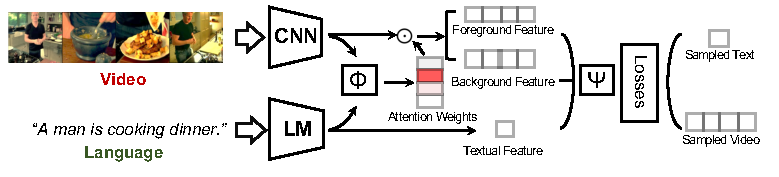
\includegraphics[width=.95\textwidth]{images/wsra_architecture.pdf}
\caption[Flowchart of the proposed \textit{WSRA}.]{\small Flowchart of the proposed \textit{WSRA}.
The losses are only used during training for temporal-textual association learning,
while inference shares the same computation flow 
for grounding textual queries over the given video. ``\textit{CNN}'' and ``\textit{LM}'' denote
video model and language model to extract features for frames and the textual query.
respectively. 
}
\label{figure:over_arch}
\end{figure}

\begin{figure*}[t]
\centering
\includegraphics[width=.95\textwidth]{images/wsra_pipeline.pdf}
\caption[ The \textit{WSRA} framework's learning losses.]{\small The \textit{WSRA} framework contains three learning losses. (a) Fore/background modelling loss forces the fore/background visual features to be discriminative by training 
over the same video \textit{w.r.t.} the ground-truth referring text $\mathbf{t}_\textit{$+$}$. (b) Video-to-text loss samples negative textual queries $\mathbf{t}_\textit{$-$}$ for each video segment for discriminative learning. The third loss is shown separately in Fig.~\ref{figure:crossvideo}.
}
\label{figure:architecture}
\end{figure*}

\subsubsection{Video-level Attention Modeling}
Prior weakly supervised methods for action localization propose to generate a weight vector to localize action labels among the video snippets in a \textit{bottom-up} manner~\citep{paul2018w,nguyen2019weakly}. While being successful in action localization from predefined categorical labels, these bottom-up methods cannot be directly tailored to the more natural language localization problem in question, as a video can correspond to multiple textual queries which appear in a very open-form language structure. Based on the fact that, the description of textual query usually covers multiple snippets in a video, we propose to model the video-level back/fore-ground features that are (ir)related to the textual query with the designed referring weights:
\begin{equation}
\begin{split}
    \boldsymbol{v}_f = &\sum^{T}_{t=1}\alpha_t\boldsymbol{v}_t \\
    \boldsymbol{v}_b = \frac{1}{T-1} &\sum^{T}_{t=1}(1-\alpha_t)\boldsymbol{v}_t,
\end{split}
\label{eq:foreback}
\end{equation}
where $v_f$ and $v_b$ are the synthesized fore/back-ground features, and weight $\alpha_t$ is calculated as:
\begin{equation}
    \alpha_t = \frac{\text{exp}(\phi(\boldsymbol{v}_t, \boldsymbol{t}))}{{\sum_{i=1}^{T}\text{exp}(\phi(\boldsymbol{v}_i, \boldsymbol{t}))}}.
    \label{eq:videoweight}
\end{equation}
In Eq.~\ref{eq:videoweight}, $\phi(\cdot, \cdot)$ is the cross-modal scoring function that measuring the distance between a frame/snippet and the textual query in the embedding space.
In practice, we define $\phi(\boldsymbol{v}, \boldsymbol{t})=\text{Sigmoid}(\text{FC}(\text{Cat}(\boldsymbol{v}, \boldsymbol{t}))$ with learnable parameters, which has a stronger association ability than cosine similarity~\citep{yu2018mattnet}, bilinear pooling~\citep{gao2016compact,fang2018modularizedtextual,kong2017low}, and second-order polynomial feature fusion~\citep{scikit-learn,gao2017tall}.
It is worth noting that the scoring function not only conveys the idea of metric learning, 
but also lands for embedding learning along with further loss terms as presented in next subsections.

As we would like to learn an embedding space in which,
1) foreground visual features tightly correspond to the given textual query measured by
the scoring function performing in the same space;
and 2) background features are clearly far away from both the foreground and textual query, as illustrated in Fig.~\ref{figure:architecture} (a).
To this end, refer to the Triplet Loss~\citep{7298682}, we set $(\phi(\boldsymbol{v}_b, \boldsymbol{t})-\phi(\boldsymbol{v}_f, \boldsymbol{t}))>m$ as our optimization target for video-level metric learning.
Rather than simply leveraging the margin or triplet-loss based contrastive learning objectiveness, we refer to the recently proposed general pair weighting framework that origins from deep metric learning~\citep{wang2020vitaa,wang2019multi}, which endows our learning objectiveness with the ability of gradient weighting using the logistic-loss as the basic form function. Comparing to the previous works as in~\citep{Mithun_2019_CVPR, chen2020look}, WSRA adaptively assigns proper weights to valuable learning pairs thus benefiting the training. 
We denote fore/back-ground similarity scores as $s_p^i=\phi(\boldsymbol{v}_f^i, \boldsymbol{t}^i)$ and $s_n^i=\phi(\boldsymbol{v}_b^i, \boldsymbol{t}^i)$, respectively. Our video-level loss function is calculated by:
\begin{equation}
    \mathcal{L}_{video} = \log\Big[1+\sum_{i=1}^{N}\exp(\gamma(s_n^i-s_p^i+m))\Big],
    \label{eq:video}
\end{equation}
in which $i$ indices the sample in a random mini-batch, $m$ is a predefined margin and $\gamma$ is a temperature factor.


\subsubsection{Snippet-level Attention Modeling}
While the above video-level loss imposed on a whole video encourages learning a discriminative embedding space and the metric functions, we introduce snippet-level modeling to enhance the contrastive study of individual video snippet and multiple textual queries, as illustrated in Fig.~\ref{figure:architecture} (b). Under this case, for the $t$-th snippet in the $j$-th video $\boldsymbol{v}_t^j$ , we calculate the referring weight $\beta_t^i$ as:
\begin{equation}
    \beta_t^j = \frac{\text{exp}(\phi(\boldsymbol{v}_t^j, \boldsymbol{t_t}))}{{\sum_{i=1}^{N}\text{exp}(\phi(\boldsymbol{v}_t^j, \boldsymbol{t_i}))}}.
    \label{eq:snippetweight}
\end{equation}



As noted, sampling semantically similar queries affect learning~\citep{wu2018unsupervised}, but when the batch size grows with limited number of textual expressions, a single training batch may contain semantically similar queries more easily,\emph{e.g.}, ``\textit{a man having food}'' and ``\textit{the man eating dinner}''. 
As a result, simply treating all other textual queries within the mini-batch as the negative samples hurt discriminative learning.
We provide our solution as below on using the similarity $(\boldsymbol{t}^i, \boldsymbol{t}^j)$ to differentiate individual instances (queries within a single
training batch), telling whether a pair of them are semantically dissimilar enough
to support a sampled negative query.




\begin{figure*}[t]
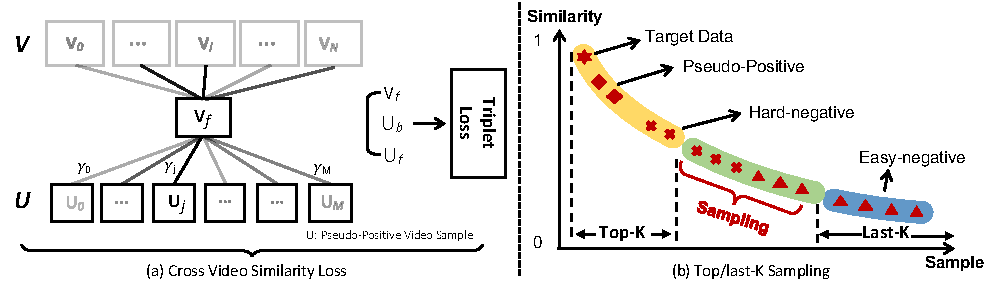
\includegraphics[width=.92\textwidth]{images/lcrov.pdf}
\centering
\caption[(a) Cross Video Similarity Loss $L_{crov}$ exploits the pseudo positive videos. (b) Demonstrative figure of queries' semantic similarity within a single training batch.]{\small (a) Cross Video Similarity Loss $L_{crov}$ exploits the pseudo positive videos, and encourage the foreground representations across samples to be similar when similar visual content occurs. (b) Demonstrative figure of queries' semantic similarity within a single training batch. The $y$-axis stands for distance measured by matching scores between
all queries and the current query in question;
$x$-axis sorts all the queries according the  matching score 
within this training batch.
%Distance represents the matching scores by computing the relevance score of the visual vector with each textual vector within the batch. 
}
\label{figure:crossvideo}
\end{figure*}
 
The negative textual queries used in the VAS loss 
are sampled within
a single training batch.
%which samples random negative textual instances within the mini-batch for the sake of learning from negative samples. 
Different with previous fore/background discriminative loss, 
VAS loss constructs a triplet as ($\boldsymbol{v}_f^i$, 
$\boldsymbol{t}^i$,
$\boldsymbol{t}^j$), 
where ($\boldsymbol{v}_f^i$, $\boldsymbol{t}^i$) are the foreground
features and corresponding (positive) textual query for the $i^{th}$ video;
and $\boldsymbol{t}^j$ is the textual query coming with the $j^{th}$ video and assumed as a negative query iff satisfying 
a condition indicated by a logic value 
${\mathbb{1}}(\boldsymbol{t}^i, \boldsymbol{t}^j)$.
We have the video-level max-margin VAS loss as below:
\begin{equation}
    \mathcal{L}_{vas} = \sum_{i=1}^{N}{\mathbb{1}}(\boldsymbol{t}^i, \boldsymbol{t}^j) \cdot 
    \text{max}(\textbf{0}, m + \psi(\boldsymbol{t}^j, \boldsymbol{v}_f^i) - \psi(\boldsymbol{t}^i, \boldsymbol{v}_f^i)).
\end{equation}
%where $\boldsymbol{t}^j$ can be the sampled negative samples within a mini-batch. 
As noted, sampling semantically similar queries affect learning~\citep{wu2018unsupervised},
but when the batch size grows with limited number of textual expressions, 
a single training batch may contain semantically similar queries more 
easily,
\emph{e.g.}, ``\textit{a man having food}'' and ``\textit{the man eating dinner}''. 
As a result, 
simply treating all other textual queries within the mini-batch as the negative samples hurt training.
We provide our solution as below on how to define ${\mathbb{1}}(\boldsymbol{t}^i, \boldsymbol{t}^j)$
to differentiate individual instances (queries within a single
training batch),
telling whether a pair of them are semantically dissimilar enough
to support a sampled negative query.





\subsubsection{Top/last-$K$ Sampling.}
Inspired by the hard negative sampling techniques in metric learning~\citep{shrivastava2016training,lin2017focal,liu2016ssd,zhang2017range}, 
we propose a top/last-$K$ sampling strategy akin to semi-hard negative sampling~\citep{schroff2015facenet}. 
We identify queries as ``pseudo-positive samples'' and ``easy-negative samples'', 
as demonstrated by Fig.~\ref{figure:crossvideo},
then we select the ``hard-negative samples'',
which provide more informative gradients that help learning.
We note ``easy-negative samples'' do not contribute to better training while being included do not hurt either yet
waste wall-clock time in computation.
To identify the ``hard-negative samples'', 
we first sort all the queries in the mini-batch based on 
the similarity scores
compared to the one given for the video of interest.
Then we simply remove the top and last $K$ samples as easy positive and negative ones.
While the hyper-parameter $K$ depends on the batch size,
we set $K=3$ in our experiments and find it quite 
stable and beneficial to the training.
%let \{$s^i_1, s^i_2 ... s^i_N$\} denotes the ranked matching scores of the video $i$, \textit{w.r.t} all textual vectors within the batch. Our negative instance $\boldsymbol{t}^j_-$ is random sampled in the set after excluding samples with relevance scores at both top and last $k$ positions, \{$s^i_{k+1}, s^i_{k+2} ... s^i_{N-k}$\} (see Figure.~\ref{figure:sample}), where $k$ is a hyper-parameter during training and depended on the batch size as well.
 
\subsubsection{Instance-level VAS Loss.}
VAS loss can be thought of a video-level multi-target learning,
\emph{e.g.}, one video with multiple textual descriptions, 
as the referring attention weights are aggregated to compute global
fore/back-ground visual features during training. 
We find further imposing a discriminative loss on individual video snippet (the instance) improves learning:
    \begin{equation}
    \label{ins-vas}
    \mathcal{L}_{ins\text{-}vas} = \sum ^{N}_{i=1}\sum^{T}_{t=1}\text{max}(\mathbf{0}, m + \alpha_{t_-}\cdot\psi(\boldsymbol{t}^i_-, \boldsymbol{v}_t^i) - \alpha_{t_+}\cdot\psi(\boldsymbol{t}^i_+, \boldsymbol{v}_t^i)),
    \end{equation}
where $\alpha_{t_+}$ and $\alpha_{t_-}$ are the referring attention weights computed by Eq.~\ref{eq:videoweight} using $\boldsymbol{t}^i_+$ (the ground-truth referring text) and $\boldsymbol{t}^i_-$ (the sampled negative text), with $\boldsymbol{v}_t^i$, 
respectively. 
We note that the weights $\alpha$ actually scales the similarity scores,
in which way the loss forces embedding learning and metric learning to be more discriminative.
%In here, the referring attention weights serve as the temperature parameters, modulating the attention weights cohere with segment-level alignment. 
We carry out ablation study on the losses in the experiment section.




% \begin{figure}[t]
% \includegraphics[width=.45\textwidth]{images/cross-video.pdf}
% \centering
% \caption{\small{Our cross video loss encourages the partial visual 
% representations across videos to be similar 
% when a common latent visual activity (if can be extracted) exists in both videos.}}
% \label{figure:crossvideo}
% \end{figure}




\subsubsection{Cross Video Similarity Loss}
%Recent efforts in in weak/un-supervision shed light upon the importance to design the learning schema that learns across instances. 
Proceeding from previous efforts in un/weak-supervised video representation learning, we are inspired with the necessity to construct contrastive learning pairs across video samples.~\citep{paul2018w} proposed to encourage the videos containing identical actions to be encoded as similar features in their corresponded temporal regions.~\citep{dwibedi2019temporal} learns the frame-wise correspondence across videos and yields great representations without any strong supervision. These works all unanimously highlight that mining the common-information among samples could enormously benefit the discriminative learning. This practice also applies for our video and language tasks, where the similar visual content can be observed in different videos. For instance, the excluded pseudo-positive samples from our VAS learning might be ``\textit{a gentleman is having dinner}'', whose visual foreground should be similar with the scenario of ``\textit{man eating food in a restaurant}''. We then exploit an inter-video loss ($L_{crov}$) for further improving the discriminativeness of learning by utilizing the mined pseudo-positive samples as stated previously. Concretely, we assume that for each target video $\boldsymbol{v}$, it contains implicit common activities with its pseudo-positive sample $\boldsymbol{u}$. Now we design our learning objective to be making their foreground representations ($\boldsymbol{v}_f, \boldsymbol{u}_f$) closer and enlarging the divergence of foreground with background ($\boldsymbol{u}_b$) as is shown in Fig.~\ref{figure:crossvideo}, where $\boldsymbol{u}_f$ and $\boldsymbol{u}_b$ is computed as the soft aggregation over all segment $\boldsymbol{u}_i$ weighted by their similarity with $\boldsymbol{v}_f$: 
\begin{equation}
    \boldsymbol{u}_f = \sum_{i}^{M} \gamma_i \cdot  \boldsymbol{u}_i.
\end{equation}
Here $M$ denotes the length of $\boldsymbol{u}$, and $\gamma_i$ represents the attention weights and are normalized by the softmax function along temporal axis:
\begin{equation}
    \gamma_i = \frac{e^{\text{cos}(\boldsymbol{u}_i, \boldsymbol{v}_f)}}{\sum_{j}^{M}e^{\text{cos}(\boldsymbol{u}_j, \boldsymbol{v}_f)}}.
\end{equation}
Since the comparing targets are from the same modality, we simply use cosine similarity as measuring function.
Our overall cross-video loss then can then be expressed as:
\begin{equation}
    \mathcal{L}_{crov} = \sum_{i=1}^{N}\lambda_i\cdot
    \text{max}(\textbf{0}, m + \frac{{\boldsymbol{u}_f^i}^T \cdot \boldsymbol{v}_f^i}{||{\boldsymbol{u}_f^i}||\cdot ||\boldsymbol{v}_f^i||} - \frac{{\boldsymbol{u}_b^i}^T \cdot \boldsymbol{v}_f^i}{||\boldsymbol{u}_b^i||\cdot ||\boldsymbol{v}_f^i||}).
    \label{equation:lcrov}
\end{equation}
We also introduce a gating parameter $\lambda_i$, which acts as the masking function that blocks out the training pairs when their textual descriptions ($\boldsymbol{t}_v, \boldsymbol{t}_u$) are not similar:
\begin{equation}
      \lambda_{i} =
    \begin{cases}
      1 & \text{if } \frac{{\boldsymbol{t}_v}^{T}{\boldsymbol{t}_u}}{||\boldsymbol{t}_v||\cdot||\boldsymbol{t}_u||} > \tau\\
      0 & \text{otherwise}\\
    \end{cases},
\end{equation}
we set $\tau=0.9$ as the similarity threshold. In such a way, we can utilize the semantic information of captions to guarantee that the constructed pseudo-positive sample is correctly chosen.
% , we found that another critical while yet under-investigated supervision comes from the cross-video samples. 
%To introduce the cross-video similarity for learned feature representations, 
% To this end,
% we initialize a random dictionary 
% $\mathbf{D} = [\mathbf{d}_1, \cdots, \mathbf{d}_C ]$
% consisting of $C$ atoms,
% which supposedly correspond to $C$ latent categories that, 
% for example, 
% describe actions or activities.
% During training,
% we also update the dictionary as described at the end of this section.
% %to contain the averagely pooled textual embedding \textit{w.r.t.} each latent class. 
% With the dictionary,
% we simply compute the cosine similarity between the textual feature with the class embedding, 
% and select the highest category as the pseudo-label. 
% Ideally, 
% we anticipate the learned visual representations across two samples to be similar in the portions 
% of videos when identical latent visual activity $\mathbf{d}_C$ occurs (see Fig.~\ref{figure:crossvideo}). 
% Our cross-video loss is defined as below:
% \begin{equation}
%     \begin{split}
%     \mathcal{L}_{crov} = \sum_{i=1}^{N}\sum_{j=1}^{C}&\uplambda_{i,j}\cdot\text{max}(\mathbf{0}, \\ 
%     m + ||{\boldsymbol{v}^i_f}{\scriptstyle[\mathbf{d}_j]} - & \boldsymbol{v}_f^+{\scriptstyle[\mathbf{d}_j]}||_2
%     - ||\boldsymbol{v}^i_f{\scriptstyle[\mathbf{d}_j]} - \boldsymbol{v}_b^+{\scriptstyle[\mathbf{d}_j]}||_2),
%     \end{split}
% \end{equation}
% where the $||\cdot||_2$ represents the Euclidean distance of two vectors, 
% $\boldsymbol{v}_f^i[\mathbf{d}]$ represents the video-level foreground feature when the referring signal is latent class embedding $\mathbf{d}$, and $\lambda_{i, j}$ is the mask function that is expressed as:
% \begin{equation}
%       \uplambda_{i,j} =
%     \begin{cases}
%       1 & \text{if } \frac{{\mathbf{d}_j}^{T}{\boldsymbol{t}^{i}}}{||\mathbf{d}_j||\cdot||{\boldsymbol{t}^{i}}||} > \tau\\
%       0 & \text{otherwise}\\
%     \end{cases}
% \end{equation}
% we set $\tau=0.9$ as the similarity threshold.
% During training, 
% class dictionary $\mathbf{D}$ is updated by averaging the matched embedding: 
% $\boldsymbol{d}_i\rightarrow(\boldsymbol{d}_i+\boldsymbol{t})/2$ in each iteration. 
% It is worth noting, 
% when $C$ increases to the number of whole training samples, 
% our cross video loss is reduced to the regular instance-level learning 
% without the notion of latent classes. 
% Essentially, 
% our cross-video loss encourages the cross-video visual features  to be similar when they share similar descriptions,
% defined by the latent dictionary being updated to cluster semantically similar textual queries.
\subsection{Overall Training Loss}
As for the overall objective loss,
we combine all the above loss terms for end-to-end training our model:
\begin{equation}
    \mathcal{L} = \alpha\mathcal{L}_{bg} + \beta\mathcal{L}_{crov} 
    + \gamma\mathcal{L}_{vas} + \delta\mathcal{L}_{ins-vas} \\
    \label{eq:overall_loss}
\end{equation}
where $\alpha, \beta$, $\gamma$ and $\delta$ are hyper-parameters weighting the loss terms.
% \shu{Shouldn't we add one sentence to say we didn't tune these hyper-parameters too much, but incrementally search over grids of choices one-by-one. refer to what we wrote in the rebuttal.}
We independently study each loss weight on top of $L_{bg}$, 
then incrementally combine all the losses and train the final model.
We list details on the use of these loss terms in the ablation study for specific tasks involved in our experiments.
During training,
we use the Adam optimizer 
with constant learning rate $10^{-4}$ and coefficients 0.9 and 0.999
for computing running averages of gradient and its square.
We implement our algorithm using PyTorch toolbox~\citep{paszke2017automatic} 
on single GTX1080 Ti GPU.

\subsection{Experiment}
The goal of our experiments is to validate the effectiveness of 
the proposed weakly-supervised framework with the top-down referring attention (\textit{WSRA}) 
for temporal-textual association learning,
through two tasks of moment localization and language grounding on
the  DiDeMo~\citep{hendricks2018localizing} and Charades-STA~\citep{gao2017tall},
respectively.
We use the mean Average Precision (mAP) 
under various Intersection over Union (IoU) thresholds to measure the performance. 
First, we elaborate on some important details about the models and language features.
We then compare our \textit{WSRA} with other state-of-the-art methods with
systematical ablation studies on the two tasks over the two benchmarks.
Finally, we visualize the qualitative results produced by our \textit{WSRA}.
% \footnote{
% Code and models will be  released
% \url{https://XXX.XXX/XXX}.}
%To show the effectiveness of our learning framework, we also conduct ablation study on the combination of various loss functions. At last, we show qualitative results of our language grounding task and analyze its future study and applications.

\noindent \textbf{Language Processing and Feature Extraction}.
The proposed  \textit{WSRA} framework is agnostic to the choice of language models.
Although one is free to use any language models providing features to represent
the textual queries (\emph{e.g.}, natural-language sentence or short phrase),   
we turn to the Openai-GPT2~\citep{radford2019language}, 
which is a released language model\footnote{\url{https://github.com/openai/gpt-2}}
trained over large-scale, diverse corpus (Wikipedia, news and books). 
% Ablation study shows that language feature extractor does not obviously benefit the performance of our model as indicated by our ablation study. 
%More specifically, we use the official released large version of GPT2\footnote{\url{https://github.com/openai/gpt-2}} (774M parameters) pre-trained on diverse corpus (Wikipedia, news and books) on the task of next word prediction. 
GPT2 is composed of a stacking of repetitive transformer modules, and we retrieve our textual features by averaging all outputs from modules as done in literature~\citep{xiao2018bertservice}.

%Note that 
%We note that, since the language features are offline, 
%the use of GPT-2 as language feature extractor does not directly benefit the performance of our model as indicated by our ablation study.
%The use of pre-trained language model is only for the consideration that it provides great sentence level representations semantically, thus enabling us to cluster the latent action dictionary precisely during training.




\subsubsection{Moment Localization on DiDeMo}

For localizing moments over a given natural-language description,
we use the Distinct Describable Moments (DiDeMo) dataset~\citep{hendricks2018localizing}, 
which includes $>$10k 25-30 second long Flickr videos. 
Manual annotations contain  $>$40k sentences with temporal boundaries 
for fine localization. 
In total, the DiDeMo dataset contains 
8,395, 1,065 and 1,004 videos for training, validation and testing respectively. We report the performances of our model on the testing split and conduct ablation studies on the validation split.
As suggested by the dataset, 
to simplify association between the sentence and a video, 
each long video is divided into 6 segments, which are annotated as whether corresponding to the sentence for localization. 
In DeDeMo, each textual description is associated with only one continuous video moment, thus yielding 21 possible candidates ($\sum_{i=1}^{6}i$). 
We measure the performance using the Rank@1 (R@1) and Rank@5 (R@5) (accuracy of the top-1/5 retrieved candidates) and their mean Intersection of Unions (mIoU) when IoU=1. To extract visual features of the videos, 
we use the official provided features 
over both RGB and optical flow~\citep{anne2017localizing}. 
For fair comparisons with other methods, as done in~\citep{hendricks2018localizing,anne2017localizing}, we compute the visual features as the concatenation of the global averagely pooled features (all 21 proposal features) and the local proposal features, which are produced by after average pooling the features from each segment.
We set hyper-parameters $\delta=1$ and $\alpha=\lambda=\gamma=0.1$ in this experiment and report results under different combinations in our supplementary materials.
During inference, we select the top-5 proposals with highest attention weights as the final prediction.

% {
% \setlength{\tabcolsep}{0.3em} % for the horizontal padding
% \begin{table}[t]
% \captionsetup{font=small}
% \centering
% \caption{Ablation study of loss terms on DiDeMo and Charades-STA dataset. 
% %The results indicate our proposed joint training yields significant improvement.
% }
% \label{table:ablation_studies}
% \small
% \begin{tabular}{cccc|ccc|ccc}
% \multirow{2}{*}{$\mathcal{L}_{bg}$} & \multirow{2}{*}{$\mathcal{L}_{vas}$} & \multirow{2}{*}{$\mathcal{L}_{ins\text{-}vas}$} & \multirow{2}{*}{$\mathcal{L}_{crov}$} & \multicolumn{3}{c|}{DiDeMo} & \multicolumn{3}{c}{Charades-STA} \\
% \cline{5-10}
% % & & & & \multicolumn{3}{c}{AP@IoU}  \\
%  &  &  & & R@1 & R@5 & mIoU & R@1 & R@5 & mIoU\\
% \hline
% \checkmark & -- & -- & --  & 12.31  & 40.03  &  22.53  & & & \\
% -- & \checkmark & -- & --  & 15.77 & 47.08  &  26.80 & & &  \\
% -- & -- & \checkmark & -- & 16.92  & 48.48  & 28.67  & & &   \\
% -- & \checkmark & \checkmark & --  & 17.50  &  48.15 & 28.97 & & &  \\
% \checkmark & \checkmark & \checkmark & --  & {17.85} & 49.28 & {29.82} & & &   \\
% \checkmark & \checkmark & \checkmark & \checkmark  &  \textbf{17.88} & \textbf{50.04}  &  \textbf{29.90} & & &  
% % \hline
% \end{tabular}
% \end{table}
% }


{
\setlength{\tabcolsep}{11.6pt} % for the horizontal padding
\begin{table}[t]
\captionsetup{font=small}
\centering
\caption{Ablation study of loss terms on the validation split of DiDeMo and Charades-STA when IoU is 1 and 0.7 respectively. 
%The results indicate our proposed joint training yields significant improvement.
}
\label{table:ablation_studies}
\small
\scalebox{.75}{
\begin{tabular}{ccc|c|ccc|ccc}
\toprule
\multirow{2}{*}{$\mathcal{L}_{bg}$} & \multirow{2}{*}{$\mathcal{L}_{vas}$} & \multirow{2}{*}{$\mathcal{L}_{ins\text{-}vas}$} & \multirow{2}{*}{$\mathcal{L}_{crov}$} & \multicolumn{3}{c|}{DiDeMo (Val)} & \multicolumn{3}{c}{Charades-STA} \\
\cline{5-10}
% & & & & \multicolumn{3}{c}{AP@IoU}  \\
 &  &  & & R@1 & R@5 & mIoU & R@1 & R@5 &mIoU\\
\hline
\checkmark & -- & -- & --  & 10.10 & 36.05  & 18.78  & 3.42 & 18.56 & 16.85\\
-- & \checkmark & -- & --  & 9.34 & 35.75 & 18.36 & 3.94 & 20.04  & 19.20\\
-- & -- & \checkmark & -- & 14.68  & 45.72  & 26.04 & 4.84 & 23.65 &22.16 \\
\checkmark & \checkmark & -- & --  & 11.76   & 39.29  & 22.41 & 4.11 & 21.88  &  18.86\\
\checkmark & -- & \checkmark & --  & 14.75  & 43.62   & 25.30  & 5.12 & 22.56  & 20.95\\
-- & \checkmark & \checkmark & --  & 15.37  &  46.26  & 27.52 & 5.81 & 23.90  & 20.55\\
\checkmark & \checkmark & \checkmark & --  & {16.20} & 49.56 & {27.50} & 7.42 & 26.65 & 24.42 \\
\checkmark & \checkmark & \checkmark & \checkmark  & \textbf{16.92}  & \textbf{50.12}  &  \textbf{28.32} & \textbf{10.05} &  \textbf{33.73} & \textbf{26.68} \\
\bottomrule
% \hline
\end{tabular}
}
\end{table}
}


% Results on DiDeMo dataset
{
\setlength{\tabcolsep}{17.6pt} % for the horizontal padding
\begin{table}[t]
\caption[Comparison of performances with fully/weakly-supervised methods on DiDeMo test split.]{\small Comparison of performances with fully/weakly-supervised methods on DiDeMo test split. Our \textit{WSRA} model outperforms the state-of-the-art weakly-supervised method (TGA)~\citep{Mithun_2019_CVPR}. We report performances of models using regular word vectors (marked as \textit{WSRA}$^{*}$). ``Chance'' denotes the results of random guess.
}
\small
\label{table:didemo}
\begin{center}
\centering
\scalebox{.75}{
\begin{tabular}{c|c|c|ccc}
% \thickhline
\toprule
\multirow{1}{*}{Supervision} & \multirow{1}{*}{Method} & \multirow{1}{*}{Feature} &
R@1 & R@5 & mIoU  \\
\cline{1-6}
& Upper Bound & -- & 74.75 &  100 & 69.05  \\
& Chance & --  & 3.75 & 22.5 & 22.64  \\
\cline{2-6} 
\multirow{6}{*}{\shortstack{\textit{Fully}\\Supervised}} & CCA & Flow\&RGB & 18.11  & 52.11 & 37.82  \\
& Lang. Obj. Retr. & {Flow}  & 16.20 & 43.94 & 27.18  \\
& LSTM-RGB-local & {RGB}  & 13.10 & 44.82 & 25.13  \\
& LSTM-Flow-local & {Flow}  & 18.35 & 56.25 & 31.46  \\
& MCN & {Flow\&RGB}  & 28.10 & 78.21 & 41.08 \\
& TGN & {Flow\&RGB}  & \textbf{28.23} & \textbf{79.26} & \textbf{42.97} \\
\hline
\multirow{5}{*}{\shortstack{\textit{Weakly}\\Supervised}}
& TGA & {Flow\&RGB}  & 12.19 & 39.74 & 24.92 \\
& WSRA  & {RGB}  & 14.20 & 43.67 & 25.22 \\
& WSRA$^{*}$ & {Flow}  & {17.23} & 48.84 & {27.42} \\
& WSRA & {Flow}  & \textbf{17.88} & 50.04 & \textbf{29.90} \\
& WSRA & {Flow\&RGB}  & 17.52 & \textbf{52.11} & 28.87 \\
% \cline{1-6}
% \thickhline
\bottomrule
\end{tabular}
}
\end{center}
\end{table}
}

To understand how each loss term contributes to the performance,
we conduct a systematical ablation study in Table~\ref{table:ablation_studies}. 
The results clearly demonstrate that all the loss terms improve the performance individually and are complementary with each other, and by combining them all achieves the best performance. Since $L_{crov}$ supervises only the visual features without any alignment, thus can not be compared independently.
From this table, it is worth noting that using the  fore/background loss only performs on par with TGA~\citep{Mithun_2019_CVPR} (see Table~\ref{table:didemo}), which is the state-of-the-art weakly-supervised method that adopts similar design of fore/back-ground modelling. 
Our final \textit{WSRA} outperforms TGA~\citep{Mithun_2019_CVPR} by a clear gain,
demonstrating that the loss terms  exploits the  weak supervision more
effectively in learning a better discriminative model.
%further distinguishes with their design that our learning pipeline includes more comprehensive weak supervisions, besides, WSRA is also trained under instance level, which is not considered by ~\citep{Mithun_2019_CVPR}. 
% We are also aware of that the inclusion of $\mathcal{L}_{crov}$
% improves quite marginally, 
% \eg, only 0.08 mIoU gain as shown in last two rows of 
% Table~\ref{table:ablation_studies}. 
% We believe this is due to  the content of the video dataset: 
% videos in DiDeMo are very diverse that are about various daily life scenes, 
% which make it difficult to exploit cross-video cues for better learning. 
% However,
% we find the cross-video loss largely boost performance  on
% the Charades-STA dataset (as shown in the next experiment),
% which contain videos for common activities. 
%In practice, we alleviate such influences by reducing the weight $\gamma$ of $\mathcal{L}_{crov}$ and also increase the number of latent classes $C$ (we found $\lambda=\beta=\gamma=0.1, C=1000$ yields satisfactory results). 
%However, we observe large performance boost by our cross-video learning mechanism in the dataset of Charades-STA (see later section), which is constructed innately upon common visual activities. 
Fig.~\ref{figure:k_sample} studies the effect of our 
top/last-$K$ sampling strategy with various $K$. 
We clearly see that, when excluding top $K=3$ and last $K=2$ samples in the mini-batch, it yields the best performance,
with the batch size set to 42 in this experiment.

\begin{figure}[t]
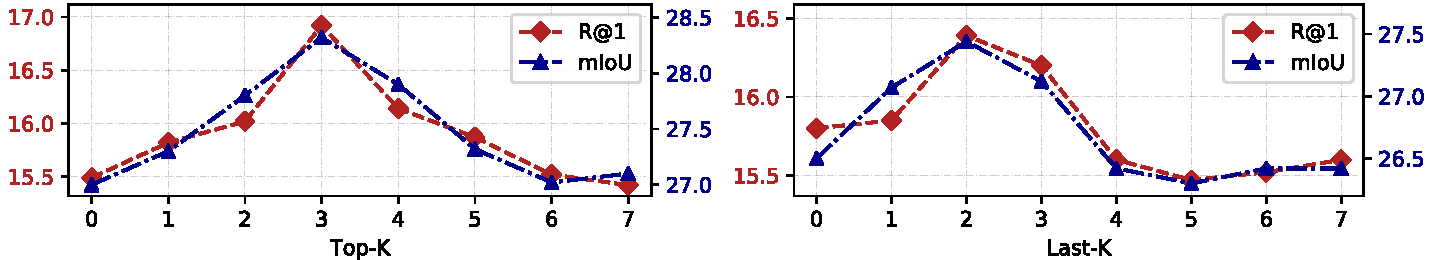
\includegraphics[width=.95\textwidth]{images/wsra_lask_K.pdf}
\centering
\caption{\small  Effect of different $K$ in the top/last-$K$ sampling on DiDeMo validation split.}
\label{figure:k_sample}
\end{figure}


% table 3
{\setlength{\tabcolsep}{.5em} % for the horizontal padding
\begin{table*}[t]
\begin{center}
\caption{ Language grounding results on the test set of Charades-STA under different intersection over unions. $^*$ denotes the work under peer reviewing.
}
\label{table:charades_sta}
\scalebox{0.75}{
\small{
\begin{tabular}{c| c | cc | cc | cc|c}
\toprule
\multirow{2}{*}{} &  \multirow{2}{*}{Approach} & \multicolumn{2}{c}{\textbf{IoU=0.3}}  & \multicolumn{2}{c}{\textbf{IoU=0.5}}  & \multicolumn{2}{c}{\textbf{IoU=0.7}}\\
 & & R@1& R@5 & R@1  & R@5   & R@1 & R@5 &  mIoU \\
\hline
\multirow{5}{*}{{\shortstack{\textit{Fully}\\Supervised}}}&Random~\citep{gao2017tall} & -- & -- & 08.51 & 37.12  & 03.03 & 14.06 & --\\
&VSA-STV \citep{kiros2015skip} & -- & --  & 10.50 & 48.43  & 04.32 & 20.21 & --\\

&CTRL~\citep{gao2017tall} & -- & -- & 21.42 & 59.11 & 07.15 & 26.91 & -- \\
&Xu \emph{et al.} ~\citep{xu2019multilevel} & -- &-- & 35.60 & 79.40  & 15.80 & 45.40 & -- \\
&MAN \citep{zhang2019man} & -- & -- & 46.53 & 86.23  & 22.72 & 53.72 & --\\

\hline 
\multirow{4}{*}{{\shortstack{\textit{Weakly}\\Supervised}}}&TGA~\citep{Mithun_2019_CVPR} & 32.14 & {89.56} & 19.94 & {65.52} & 08.84 & 33.51 & --\\
&SCN~\citep{lin2019weakly} &  42.96 & \textbf{95.56}  & 23.58 & \textbf{ 71.80}& 09.97 & {38.87} & --\\
&CTF$^{*}$~\citep{chen2020look} &  39.80 & - &  27.30 & - & \textbf{12.90} & - & --\\
% &WSRA-\textit{Verb}  & 46.50 & 73.84 & 29.35 & 60.48  & 10.05 & 33.73 & 29.05 \\
% &WSRA-\textit{Lang} & 43.63 & 73.58  & 27.02 & 55.62 & 08.87 & 26.91 & 26.68  \\
&WSRA (Ours) & \textbf{50.13} & {86.75}  & \textbf{31.20} & 70.50& {11.01} & \textbf{39.02 }& \textbf{31.00} \\
\bottomrule
\end{tabular}
}
}
\end{center}
\end{table*}
}

We compare our \textit{WSRA}  with other advanced weakly/fully-supervised methods in Table.~\ref{table:didemo}. 
As the previous methods, 
we experiment with visual features from modals of RGB and optical flow. 
Upper-bound of DiDeMo is brought since the human annotators cannot achieve 100\% agreement in 
annotating the segment boundaries \emph{w.r.t} the given video-level sentence~\citep{anne2017localizing}.
Comparing with the baseline models, 
our \textit{WSRA} model  significantly outperforms weakly supervised TGA~\citep{Mithun_2019_CVPR} by 5.5\%, 11\% at R@1 and R@5 respectively, 
even achieving comparable performance with several fully supervised methods \emph{e.g.}, CCA~\citep{anne2017localizing} and LSTM based model~\citep{anne2017localizing}. 
It is also worth noting that, our \textit{WSRA} model has similar number of parameters with all above mentioned baseline models. 
% In Fig.~\ref{figure:didemo}, we exhibit examples of the grounding attention weights together with a failure case.
% We notice that \textit{WSRA} shows high attention on the video segment that corresponds to the query. However in the second case, \textit{WSRA} fails to distinguish the video segments as the attention weights show similar values. This can be partly ascribed to the extremely alike visual contents of the video, which prevents the model from associating the descriptions with a distinct moment.



\subsubsection{Language Grounding on Charades-STA}
We further validate our \textit{WSRA} for the language grounding task on another video dataset, 
Charades-STA~\citep{gao2017tall},
which augments the Charades dataset~\citep{actorobserver,sigurdsson2017asynchronous}  with
manual annotations in the form of 
natural language descriptions at precise start-end timestamp of each video.
Charades-STA contains 12,408/3,720 video-query pairs for training/testing. 
For annotation,
Charades-STA expands each verb to generate a textual sentence
from single caption in Charades using language templates, 
and associate the sentence with frames corresponding to this verb.
To encode the video segment,
as done by other weakly-supervised methods 
for action localization~\citep{nguyen2018weakly,paul2018w},
we use the I3D feature from a pre-trained model trained over 
the Kinetics dataset~\citep{carreira2017quo}. 
For inference, we turn to the moment selection methods~\citep{gao2017tall},
which generate multi-scale sampled moment candidates using sliding window method for retrieval with fixed length of frames. 
Moreover, 
since the  video duration varies significantly, we sampling the moment 
candidates with lengths proportioned to the video duration.
Specifically, sampled candidate clips are with $\small\{$20\%, 30\%, 40\%, 50\%$\small\}$ of the whole videos and in 80\% overlap using the sliding window manner, then the moment with highest attention weight score is selected as the final prediction. More details can be found in the supplementary.
\begin{figure*}[t]
\includegraphics[width=.98\textwidth]{images/wsra_qualitative.pdf}
\centering
\caption{\small Qualitative examples of the language grounding on Charades-STA dataset. We select the top several video moments with high attention weights as the prediction.}
\label{figure:qualitative}
\end{figure*}
% \begin{figure*}[t]
% \includegraphics[width=1.0\textwidth]{images/retrieval.pdf}
% \centering
% \caption{\small Examples of the sampled ``pseudo-positive'' videos, where exist the common activity of ``\textit{watching tv}'', and irrelevant videos in a batch that serves as negative samples for learning.}
% \label{figure:sampled}
% \end{figure*} 
We report the performance comparison with
different mean Intersection-over Union (mIoU = \{0.3, 0.5, 0.7\}) and Recall@\{1, 5\}, 
and the mIoU as a summary metric.
We list detailed comparison in Table~\ref{table:charades_sta}.
From our \textit{WSRA} and TGA~\citep{Mithun_2019_CVPR}, 
we can see the clear advantage of our referring attention:  
\textit{WSRA} significantly outperforms TGA, 
for example by 18\% at [R@1, IoU=0.3], 
and 12\% at [R@1, IoU=0.5], respectively. 
We can also see clearly from the above table that, 
\textit{WSRA} demonstrates either comparable or even better performance than 
most fully-supervised methods. 
% In right side of Fig.~\ref{figure:sampled}, we showcase examples of the sampled videos during learning, our cross-video loss enables the \textit{WSRA} to exploit the common activity exist in both videos. 
In the meanwhile, our top/last-$K$ sampling also rejects theses pseudo-positive and less informative samples in the contrastive learning. Fig.~\ref{figure:qualitative} shows the qualitative examples of grounding in Charades-STA dataset where the moment is aligned with language query even facing much longer videos. We further study the effect of cross-video loss in the supplementary.
% \begin{figure*}[t]
% \centering
% \includegraphics[width=.90\textwidth]{images/didemo.pdf}
% \caption{\small We show the attention weights of language grounding on DiDeMo with a failure example. Ground-truth moment is in red-box.}
% \label{figure:didemo}
% \end{figure*}
\subsection{Conclusion}
In this paper, we propose the weakly supervised model with the referring attention mechanism (\textit{WSRA})  for learning temporal-textual association on videos.
We introduce several novel loss terms and sampling strategies,
all of which help better learning by fully exploiting the cues from 
the weak supervision at video level.
Through extensive experiments on two benchmarks,
we show the \textit{WSRA} model outperforms the state-of-the-art weakly-supervised
methods by a notable gain,
achieving on par or even better performance than some fully-supervised methods. As an outlook for the future study, we consider that the most potential aspect our model would benefit comes from the video-language representation learning at scale~\citep{miech2019howto100m}, whereas the training is often severely accompanied by uncurated annotations: \textit{e.g.}, temporally misaligned descriptions~\citep{miech2019end}. To construct a soundly and largely pre-trained model, it is requisite to properly leverage the weak or biased annotation at comprehensive views. Our \textit{WSRA} provides us with such a perspective as the trailblazer, that investigates thoroughly how language can be fully exploited as valid supervisions even without temporal annotations.